\section{Introduction}

Modern society seamlessly adapted to using gadgets and appliances that 30 year ago only existed in futuristic science fiction movies. Smart devices have slowly become part of everyday lives. Self driving trucks are not something out of a distant future anymore\cite{freedman_2017} and Internet connected appliances such as light bulbs and  smart coffee makers are finding their places in common people homes. It was estimated that in 2017 there were around 27 billion connected IoT devices around the globe. This number is expected to increase by around 12 \% each year until it reaches 125 billion by 2030 \cite{ihs-markit}. For comparison in 2014 there were around 1.57 billion smart phone owners worldwide, this number is bound to reach 2.87 billion by 2020 \cite{statista}. Although, smart phone numbers are growing fast, they are limited by the number of people using them. This is not the case with smart Internet of Things devices. For example an industrial factory may contain hundreds of different sensors. The IoT networks and stand-alone "Smart things" technologies are booming \cite{gartner2018} and will only increase in numbers. Unsurprisingly, such growth is starting to cause privacy, security and regulation concerns as it is hard to control. Even though these technologies have greatly complimented people lives one can not stop wonder are their owners properly manage these numbers of Internet connected devices.

Even though IoT devices collect incredible amount of users sensitive information and it is starting to cause processing and security concerns \cite{7069995} little is being done to properly secure these devices. As it has been shown by the Mirai botnet attack in 2016, IoT technologies can be used to create record breaking botnets and disrupt more traditional Internet services\cite{203628}. If proper measures are not taken it is likely that more large scale malicious IoT network exploitation will take place. As the manufacturers are pushed by market growth to develop new products faster in order to keep up with their competitors proper security testing is becoming luxury that usually can not be afforded. Moreover, it appears that consumers are not concerned about their device security\cite{iotm}. As studies have shown even Internet connected vehicles can be hacked into and controlled remotely\cite{8071577}. As Internet connected devices are exposed to many more threats than a non-connected electronic devices steps must be taken to ensure IoT gadgets and Internet connected devices are robust and safe to use.

Due to vast differences in deployment environment as well as technologies in use proper IoT technology testing is difficult to ensure. One reason severely complicating the testing process is the use of third-party technologies and services. A single IoT device firmware may be written by a mix of contracted developers known as Original Design Manufacturers (ODM) and in-house developers hired by hardware manufacturer Original Equipment Manufacturer (OEM), then the application code itself may be supplied by a completely different company\cite{cookbook}. The problem occurs when OEM and ODM merge code bases. The ODM may provide only the binary files or an SDK for the OEM. Therefore, if that happens Original Equipment Manufacturer which is responsible for distributing firmware, managing it and releasing updates, does not have full access to the code. Moreover, IoT networks are comprised of many different kinds of devices that are responsible for different functions. Each individual device may be manufactured by different suppliers and their OEMs accordingly. As no individual link of the supply chain posses access to the full infrastructure source codes, it may be impossible to thoroughly test the system as a whole. It becomes apparent that black box type penetration testing and vulnerabilities scan may be the only acceptable strategy in order to secure complicated IoT systems.

As the field in question is rather new, diverse and rapidly developing it is complicated to find knowledgeable specialists and tools developed specifically for IoT penetration testing. There are numerous blogs and projects offering various level of detail guides to IoT penetration testing\cite{github}. Some organizations including IEEE and ETSI have released technology-specific standards as well as security guidelines but non try to cover IoT in general\cite{Zhao:2013:SIT:2584913.2585964}. 

The purpose of this project is to try to simplify IoT penetration testing. It summarizes the general concepts of IoT penetration testing and present them in a user friendly manner. Moreover, this project tries to address the lack of dedicated IoT penetration testing technologies and provides an extendable framework which purpose is to reuse existing penetration tools to test IoT systems. The tool is designed to require little technical knowledge and is highly modifiable in order to adapt to particular IoT infrastructure.

This report is divided into sections starting with an abstract and introduction. The subsequent parts of this report background research and investigates the most commonly used IoT technologies and protocols up-to-date. Afterwards, distinct goals and requirements are listed for this project. They are followed by explanation of design decisions and the general structure of the application. This report is finalized by listing remaining work and explaining project management decisions taken up to this point.

\section{Background research}
There is no clear definition of the Internet of Things technologies. Some define it as "the concept of every device blending with the existence of human beings"\cite{DBLP:journals/corr/MendezPY17}. Which basically means that there would be no difference between human and device interaction with the system. In it's simplest form IoT systems can be defined as decentralized networks there multiple, usually, limited capabilities embedded processing units communicate between each other in various ways. The fact that they have communication capabilities implies that they can change their behaviour depending on input received via network. That is what exposes "smart objects" to outside threats\cite{riahi:hal-00868362}. This increases the penetration testing complexity from a single isolated embedded device to a distinct Internet entity that requires a new layer of security. Addition of a network interface transforms a narrow purpose device into an interactive network component.

Insertion of previously isolated technologies into the global Internet network attracts malicious users attention. Unprotected log-ins, outdated software and insecure communication would not cause major security issues for hidden away, stand-alone embedded devices as long as they function properly (e.g. medical equipment). The situation is the opposite if a device can be discovered and interacted with by anyone on the network. Moreover, IoT devices can be extremely favourable targets to hackers which are expanding their bot networks. Unlike regular computers, IoT devices usually run continuously without halting and can be exploited without owners knowledge\cite{191952}. It seems that traditional approaches of securing devices are not effective\cite{DBLP:journals/corr/abs-1803-05022} due to IoT technologies uniqueness and variety.

Above listed problems require penetration testing to be taken in several layers, breaking down IoT network infrastructure and exposing separate attack vectors. Testers must take into account 6 different aspects of IoT infrastructure. Hardware vulnerabilities can be exploited by anyone who has physical access to the device. Such vulnerabilities may be an open debugging port, password reset button and tapping into hardware level communication (e.g. UART)\cite{attify}. Firmware in this context stands for device operating system which can be rather primitive or extensive and using third party SDK and libraries introducing possible vulnerabilities\cite {cookbook}. Application level vulnerabilities usually happen due to a software bug or a logic error\cite{cookbook}. Communication and network exploits happen due to man-in-the-middle attacks and usage of insecure communication protocols assuming security by obscurity. If a device or an IoT system has a web interface, it essentially becomes a web host, thus it may have all the vulnerabilities of a regular website\cite{2007:WAH:1406550}. Lastly, some IoT vendors release mobile applications complimenting their products. That is another new and troublesome attack vector as hackers may get access not only to victims IoT devices but also get a foot hold in user smart phone possibly accessing sensitive information stored in there\cite{cookbook}. Only by addressing each part of the infrastructure individually and as a whole one can truly secure IoT systems.

The most popular and the most convenient method to interact with an IoT device is via wireless network. There are many different communication technologies developed for this purpose. All of them were designed to accomplish specific tasks, therefore they vary in range, connection speed, energy consumption and security. Some of the most widely used are WiFi, Bluetooth, ZigBee, GSM and Z-Wave \cite{cookbook}. To devise a proof of concept, two different protocols are sufficient, therefore this project will concentrate on WiFi and Bluetooth communication. WiFi is based on IEEE 802.11 standards, it is no different to LAN communication. The two most ways of sending information is UDP and TCP protocols which act very differently \cite{4359944}. By itself WiFi communication is not encrypted, therefore if application developers did not secure ongoing traffic, such data is vulnerable to network sniffing attacks. Recent versions of Bluetooth, contrarily have built-in encryption, therefore sniffing it is rather complicated \cite{scarfone2012guide}. Nevertheless, Bluetooth devices are still vulnerable when they connect to an end-point for the first time (pairing) \cite{scarfone2012guide}. It is easier to exploit specific protocol vulnerabilities with tools already designed for that purpose. As the tool set is designed to take re-use best parts of already trusted penetration tools, it will be able to retain generality still succeeding in fine-grain testing.

\subsection{Threat modelling}
According to the "IoT Penetration Testing Cookbook"\cite{cookbook} threat modelling can be broken down into these steps:
\begin{enumerate}
    \item Document all system assets using publicly available information: try to identify each device, write down all applicable information that may provide any hints on systems internal processes.
    \item Create architecture overview:
    \begin{itemize}
         \item Document IoT system functionality and features, create use cases
         \item Create architectural diagram that shows what components control flow
         \item Using architectural diagram and created use cases identify each individual component and communication method system communication method.
    \end{itemize}
    \item Use acquired system picture to identify entry points and write down possible threats. It does not have to be exact but it has to be backed up by some evidence.
    \item Starting with most likely threats determine:
    \begin{itemize}
        \item Threat targets 
        \item Possible exploitation techniques
        \item Possible countermeasures
    \end{itemize}
    \item Rate threats using DREAD rating system\cite{dread} and group them accordingly (High 12-15, Medium 8-11, Low 5-7)
    \item After the overall system analysis is finished, repeat the same process examining each part of the IoT system separately. Reuse previously created mapping and include new information reflecting on device specific threats. This is the time to logically and realistically evaluate each part of the system.
    Writing down possible threats for individual devices, mapping attack surfaces and identifying vulnerabilities which may lead to exploitation of distinct device weaknesses.
    \item Final step is to analyze and attack top ranking vulnerabilities of each system component (firmware, mobile application, communication, etc.) looking for a way in.
\end{enumerate}


\section{Project Goals}
This project goal is to collect information about IoT penetration testing and provide a tool that allows the generalized methodology to be easily applied in practise. The tool should be able to execute different types of network scans and display discovered devices in a user-friendly manner. The tool is also supposed to be able to apply information gathering techniques to individual devices such as port scanning. The idea is to visually present device and network specific information gathered from automatic and manual tests to get a better understanding of the system. By following penetration testing methodology it is then possible to identify attack surfaces and exposed entry points.

With initially gathered information a user can then choose one of the modular tools added to the application and apply device or protocol specific tests. The biggest advantage of a tool like this is its ability to use preexisting penetration tools to achieve individual tasks. As the IoT technology stack is so diverse it is impossible to design a tool that covers all the use cases. Instead, this project should provides a "tool box" which comes with a few basic testing tools and ability to add new tools if a need arises. The basic tools allow users to get a first view at the system of interest and make decisions about the next step.

As one of the emphasis of this application is to make IoT penetration testing more accessible and coherent for a diverse audience the ease-of-use and simplistic design are key aspects of the application. The whole tools functionality needs to be accessible via a graphical user interface with hints and explanations reducing the learning curve.

\subsection{Requirements}
    \subsubsection{Functional}
        \begin{itemize}
            \item Functionality to add and remove new security tools to and from the application
            \item Contain an initial proof-of-concept set of tools
            \item Scan local network, map network infrastructure and identify its components
            \item Support at least 2 communication protocols: WiFi and Bluetooth
            \item Provide guidelines and best practice for IoT penetration testing
            \item Give suggestions of most likely vulnerabilities in response to the initial network scan
            \item Allow chaining separate tool execution
            \item User is able to interact with the application via a graphical user interface
        \end{itemize}
    
    \subsubsection{Non-functional}
        \begin{itemize}
            \item Contains all required dependencies and is portable with little to no setup
            \item Compatible with most popular Linux distributions
            \item Must provide user with feedback within 2 second of user interaction
            \item Must be able to identify at least 25 unique devices on the network
        \end{itemize}

\subsection{Limitations}
This project cannot possibly find all existing IoT device vulnerabilities nor address specific firmware or hardware details; thus, it will only check for most frequent IoT device weak points. The tool set concentrates on finding application and communication level vulnerabilities. Some communication protocols may require special hardware tools and are harder to test. Because of the modular nature of the application design it may be possible to use such tools e.g. for capturing GSM communication packages \cite{DBLP:journals/corr/ShaikBANS15} but due to time and resource limitations it is out of scope of this module. It is also impossible to use the same technique to test an area as diverse as IoT networks. Therefore, the methodology provided is only guidelines gathered from multiple sources and may need alterations.

\subsection{Risk analysis}
Probability and Impact are rated in a scale from 1 to 5.

\def\riska{Loss of source code at some stage of development}
\def \probabilitya {1}
\def \impacta {4}
\def \mitigationa {Use of remote source control  repository to frequently record every stage of the development, thus being able to recover it if needed. }

\def\riskaa{Unable to fulfill all of the requirements due to technical implemention difficulties}
\def \probabilityaa {3}
\def \impactaa {2}
\def \mitigationaa {During the start of development process requirements will be split into tasks, divided into sprints and ranked using Agile methodology, therefore ensuring that core functionality will be implemented first and a working proof of concept is available at the end of the project }

\def\riskaaa{Loss of development time due to other course modules}
\def \probabilityaaa {2}
\def \impactaaa {2}
\def \mitigationaaa {Dedicate fixed amount of time every week for the project in order to keep up with the schedule }

\def\riskaaaa{Some part of the project taking up significantly longer that expected}
\def \probabilityaaaa {3}
\def \impactaaaa {2}
\def \mitigationaaaa {Re-evaluate task importance and readjust development schedule in order to deliver functional prototype }

\def\riskaaaaa{Unable to complete adequate application testing due to technical or time limitations}
\def \probabilityaaaaa {3}
\def \impactaaaaa {3}
\def \mitigationaaaaa {Complete limited or partial testing concentrating on core functionality, document causes and reasoning. If difficulties arise in early stages of development  due to technical limitations, seek support from university staff that have more experience in similar situations. }

\begin{center}
\begin{tabular}{ |m{5cm}|m{2cm}|m{1cm}|m{6cm}| } 
 \hline
 Risk & Probably & Impact & Mitigation \\ 
 \hline
 \riska & \probabilitya & \impacta & \mitigationa \\ 
 \hline
 \riskaa & \probabilityaa & \impactaa & \mitigationaa \\ 
 \hline
 \riskaaa & \probabilityaaa & \impactaaa & \mitigationaaa \\ 
 \hline
 \riskaaaa & \probabilityaaaa & \impactaaaa & \mitigationaaaa \\ 
 \hline
 \riskaaaaa & \probabilityaaaaa & \impactaaaaa & \mitigationaaaaa \\ 
 \hline
\end{tabular}
\end{center}



\section{Application design}
The penetration testing tool is chosen to be a desktop based GUI application. Desktop applications will have no dependencies on browsers. Server side - client side code complications and JavaScript engine dependencies are also removed. It is planned that all libraries and resources required for the application to run would be included in the final deliverable, thus increasing portability and reducing setup complexity. Additional features as automatic update service and application error scan is planned in order to keep software up to date by using git repository as a code base.

Application will implement modular design to re-use existing penetration tools and follow usage-centered design principles. In order to add a tool to the tool set, a user will have to define an interface/wrapper for the new tool. The wrapper will contain instructions on how to convert GUI input to tool specific commands as well as interpret tools output. This design allows flexibility and makes no assumptions about individual tool input or output. By prioritizing usability and clarity the application will remain user friendly and minimize new users learning curve \cite{user}.

It has been decided that the application will be written in Python. Python is a dynamic scripting language suitable for rapid development and prototyping. There will be no learning curve to use it as work experience is already present. Graphic User Interface will be developed using PyQT library as it is highly customize and popular between Python developers. Python is also by default present in the majority of Linux distributions, therefore no additional setup will be required. Other alternatives as Java, JavaScript and C++ were considered but were dismissed due slower development cycle, steeper learning curve or lack. One may point out Python lesser performance as a disadvantage but as the majority of computationally heavy tasks will be executed by other tools that does not make any difference.

A UML diagram present describes general application structure.

\begin{figure}[h!]
\caption{UML diagram}
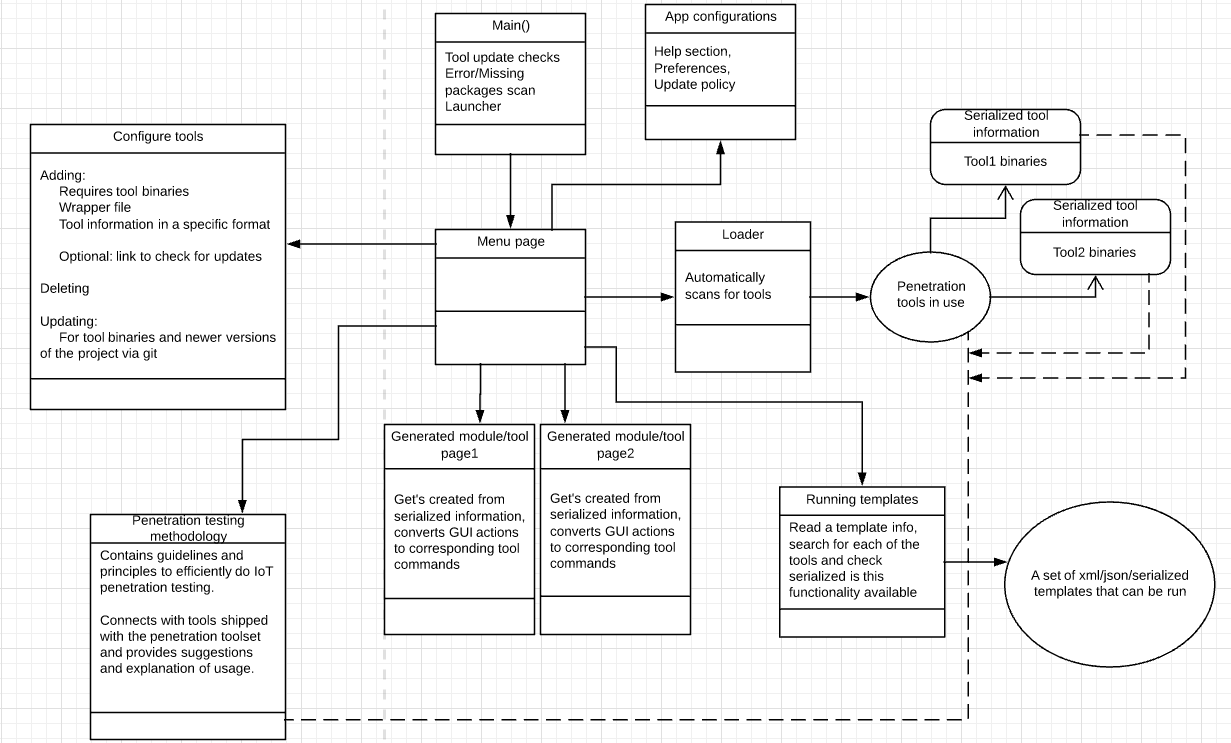
\includegraphics[width=\linewidth]{UML-diagram}
\centering
\end{figure}

\section{Remaining work}

Work completed up to this point and the remaining work is visualized using Gannt chart. The application design and background research phases are completed. The remaining development time will be mostly divided into sprints of 10-14 days in order to assign time for inevitable other module assignments. Each sprint will have a predefined set of tasks prioritized in Agile manner. After the sprint is completed planned functionality is supposed to be fully functional and tested to constantly add value. The Christmas period, January exam period and Easter periods are planned in looser manner in order to accommodate vacations, assess progress and re-think design decisions. The last weeks of the project are reserved for writing final report.

\begin{figure}
\caption{Gannt chart}
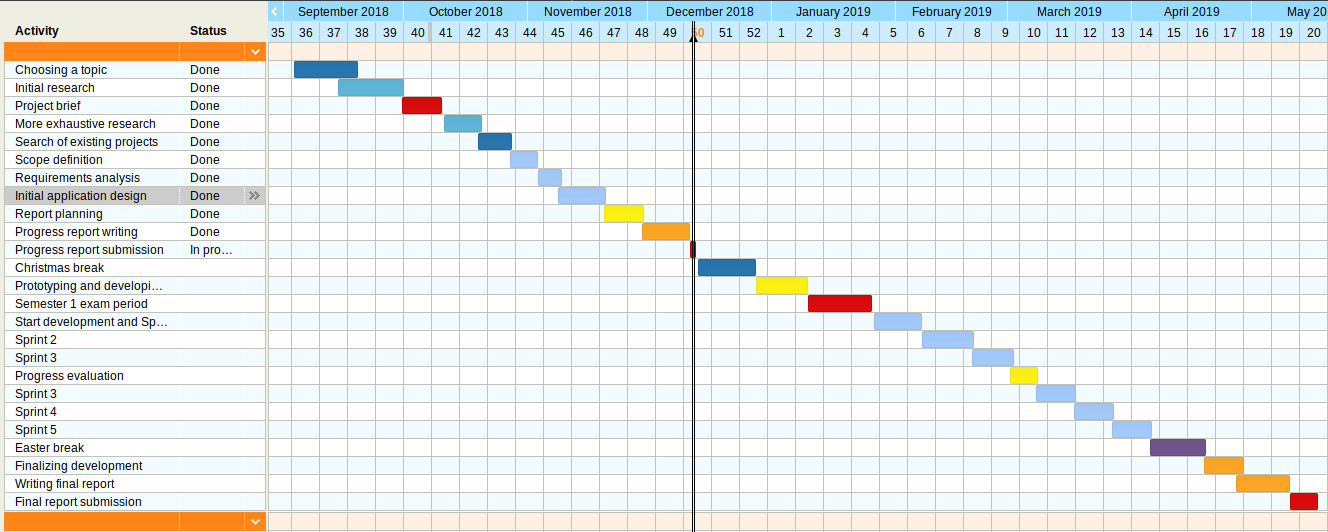
\includegraphics[width=\linewidth]{Gannt}
\centering
\end{figure}